\subsection{Obiettivo e configurazione}

La campagna E1 isola il solver prima di interpretare i confronti di mesh movement. Sono stati mantenuti PDE manufatta, forzante, condizioni iniziali e al contorno e coefficienti fisici del benchmark principale. La discretizzazione è Galerkin $P_1$ con backward Euler. La campagna include: (i) convergenza temporale su mesh $32\times32$; (ii) convergenza spaziale su tre mesh con un indicatore di contaminazione temporale; (iii) statistiche locali del numero di Péclet; (iv) confronto Galerkin/SUPG; (v) verifica indipendente della D-GCL; (vi) work--precision su mesh fisse.

\subsection{Convergenza temporale}

Per backward Euler ci si attende un errore temporale di primo ordine, sotto le usuali ipotesi di regolarità e quando l'errore spaziale è sufficientemente piccolo da non dominare la differenza osservata. La stima dell'ordine è ottenuta dalle differenze tra soluzioni con passi dimezzati sulla stessa mesh, non soltanto dal confronto con la soluzione esatta. Gli ordini Cauchy osservati sono 0.943, 0.969 e 0.983 passando rispettivamente da $\Delta t=0.01$ a $0.005$, da $0.005$ a $0.0025$ e da $0.0025$ a $0.00125$. La progressione è coerente con il regime di primo ordine previsto, pur non essendo una dimostrazione asintotica uniforme rispetto a tutte le risoluzioni.

\begin{table}[tbp]
\centering\small
\caption{Convergenza temporale del solver Galerkin $P_1$ su mesh $32\times32$. L'ordine è stimato dalle differenze Cauchy tra passi dimezzati.}
\label{tab:e1_temporal}
\begin{tabular}{rrrr}
\toprule
$\Delta t$ & Passi & Differenza Cauchy $L^2$ & Ordine osservato $q$\\
\midrule
0.01000 & 50  & $4.672\times10^{-3}$ & --\\
0.00500 & 100 & $2.431\times10^{-3}$ & 0.943\\
0.00250 & 200 & $1.242\times10^{-3}$ & 0.969\\
0.00125 & 400 & $6.283\times10^{-4}$ & 0.983\\
\bottomrule
\end{tabular}
\end{table}

\begin{figure}[H]
\centering
\IfFileExists{images/stage_e/temporal_convergence.pdf}{%
  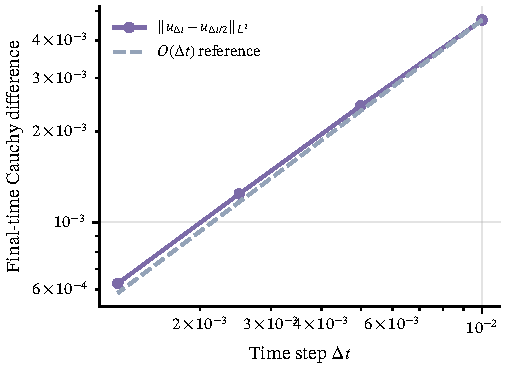
\includegraphics[width=0.95\columnwidth,height=0.29\textheight,keepaspectratio]{images/stage_e/temporal_convergence.pdf}%
}{%
  \fbox{\begin{minipage}[c][0.105\textheight][c]{0.88\columnwidth}
  \centering\footnotesize\textbf{Figura non inclusa nel pacchetto sorgente}\par\vspace{0.35em}
  \scriptsize\nolinkurl{images/stage_e/temporal_convergence.pdf}
  \end{minipage}}%
}
\caption{Convergenza temporale del solver Galerkin su mesh $32\times32$; le differenze Cauchy mostrano un ordine osservato che si avvicina a uno.}
\label{fig:e1_temporal}
\end{figure}

\subsection{Convergenza spaziale e separazione spazio--tempo}

La Tabella~\ref{tab:e1_spatial} riporta le norme assolute medie nel tempo degli errori $L^2$ e della seminorma $H^1$. Gli ordini osservati sono calcolati tra livelli consecutivi. Per evitare di attribuire al raffinamento spaziale una riduzione dovuta al passo temporale, è stato inoltre calcolato il rapporto tra la differenza temporale Cauchy sulla stessa mesh e l'errore assoluto medio della soluzione a passo più fine. Tale rapporto è un indicatore operativo di contaminazione, non una stima rigorosa superiore dell'errore temporale.

\begin{table*}[!t]
\centering\small
\caption{Convergenza spaziale e indicatore operativo di contaminazione temporale. Gli errori sono assoluti e mediati nel tempo; la soglia predefinita per la contaminazione è 10\%.}
\label{tab:e1_spatial}
\begin{tabular*}{\textwidth}{@{\extracolsep{\fill}}rrrrrrr}
\toprule
Griglia & DOF & $E_{L^2}$ & $p_{L^2}$ & $|e|_{H^1}$ & $p_{H^1}$ & $\rho_t$\\
\midrule
$16^2$ & 289  & $9.871\times10^{-3}$ & -- & $7.017\times10^{-1}$ & -- & 1.55\%\\
$32^2$ & 1089 & $2.573\times10^{-3}$ & 1.940 & $3.574\times10^{-1}$ & 0.973 & 6.66\%\\
$64^2$ & 4225 & $7.216\times10^{-4}$ & 1.834$^\dagger$ & $1.743\times10^{-1}$ & 1.036$^\dagger$ & 24.05\%\\
\bottomrule
\end{tabular*}
\vspace{0.25em}
\parbox{0.98\textwidth}{\footnotesize $^\dagger$ L'ordine tra $32^2$ e $64^2$ è riportato come valore osservato, ma non è considerato spazialmente isolato perché $\rho_t$ supera la soglia del 10\%. La coppia $16^2$--$32^2$ soddisfa il criterio operativo; la convergenza spaziale non è pertanto ancora chiusa su tre livelli.}
\end{table*}

Per $P_1$ e una soluzione sufficientemente regolare ci si attende asintoticamente $E_{L^2}=O(h^2)$ e $|e|_{H^1}=O(h)$. La coppia $16^2$--$32^2$ fornisce ordini osservati rispettivamente 1.94 e 0.97, compatibili con queste attese nel regime considerato. Il livello $64^2$ ha errori inferiori, ma il rapporto di contaminazione 24.05\% supera il criterio operativo del 10\%; il suo ordine non viene quindi usato come conferma conclusiva e il livello è escluso dall'evidenza di convergenza spaziale isolata. La verifica E1 supporta quindi un ordine spaziale indicativo sulla coppia $16^2$--$32^2$, non una dimostrazione su tre livelli.

\begin{figure}[!htbp]
\centering
\IfFileExists{images/stage_e/spatial_convergence.pdf}{%
  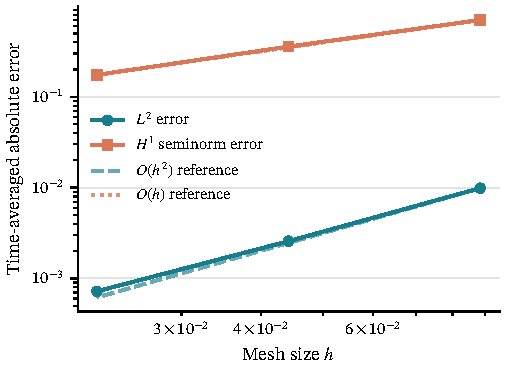
\includegraphics[width=0.95\columnwidth,height=0.29\textheight,keepaspectratio]{images/stage_e/spatial_convergence.pdf}%
}{%
  \fbox{\begin{minipage}[c][0.105\textheight][c]{0.88\columnwidth}
  \centering\footnotesize\textbf{Figura non inclusa nel pacchetto sorgente}\par\vspace{0.35em}
  \scriptsize\nolinkurl{images/stage_e/spatial_convergence.pdf}
  \end{minipage}}%
}
\caption{Errori assoluti medi nel tempo e ordini osservati per il raffinamento spaziale; il livello $64\times64$ è evidenziato come contaminato temporalmente secondo il criterio adottato.}
\label{fig:e1_spatial}
\end{figure}

\subsection{Numero di Péclet locale}

Il numero di Péclet è calcolato per elemento usando la velocità relativa alla mesh $\boldsymbol\beta=\bm b-\bm w$:
\begin{equation}
Pe_K=\frac{\norm{\boldsymbol\beta}\,h_K^{\beta}}{2\nu},\qquad
h_K^{\beta}=\frac{2\norm{\boldsymbol\beta}}{\sum_i|\boldsymbol\beta\cdot\nabla\varphi_i|},
\label{eq:peclet_local}
\end{equation}
con il limite $Pe_K=0$ quando la velocità relativa è nulla. Per la mesh fissa, $\bm w=0$ e $Pe_K=7.8125$ per tutti gli elementi della griglia strutturata. Per ALE la distribuzione varia con il tempo e con la deformazione. Al tempo $t=0.25$, la mediana è 8.91, il 95-esimo percentile 10.84 e il massimo 11.11. La variabilità locale mostra perché un solo valore globale non descrive completamente il regime convettivo della mesh mobile.

\begin{table}[tbp]
\centering\small
\caption{Statistiche del numero di Péclet element-wise per il solver ALE. Per la mesh fissa il valore è costante e pari a 7.8125 in tutti gli istanti.}
\label{tab:e1_peclet}
\begin{tabular}{rrrr}
\toprule
$t$ & Mediana & 95-esimo percentile & Massimo\\
\midrule
0.000 & 6.883 & 7.740 & 7.813\\
0.125 & 8.640 & 10.256 & 10.514\\
0.250 & 8.910 & 10.839 & 11.106\\
0.375 & 7.149 & 7.934 & 8.233\\
0.500 & 6.855 & 7.738 & 7.813\\
\bottomrule
\end{tabular}
\end{table}

\begin{figure}[!htbp]
\centering
\IfFileExists{images/stage_e/peclet_distribution.pdf}{%
  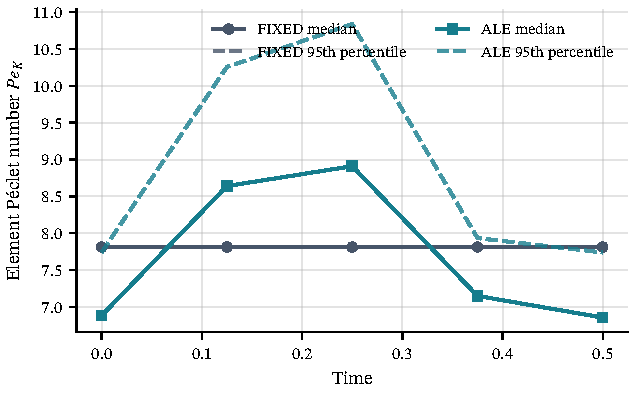
\includegraphics[width=0.95\columnwidth,height=0.29\textheight,keepaspectratio]{images/stage_e/peclet_distribution.pdf}%
}{%
  \fbox{\begin{minipage}[c][0.105\textheight][c]{0.88\columnwidth}
  \centering\footnotesize\textbf{Figura non inclusa nel pacchetto sorgente}\par\vspace{0.35em}
  \scriptsize\nolinkurl{images/stage_e/peclet_distribution.pdf}
  \end{minipage}}%
}
\caption{Distribuzioni del numero di Péclet locale su mesh fissa e ALE in diversi istanti temporali.}
\label{fig:e1_peclet}
\end{figure}

\subsection{Confronto Galerkin e SUPG}

La variante SUPG è stata confrontata con Galerkin a $32\times32$ e $\Delta t=0.0025$, sia su mesh fissa sia in ALE mobile. Il moto usato nella colonna ``Moving ALE'' è una deformazione armonica prescritta, indipendente da GDM e dai controllori MMPDE. Posto $\psi(x,y)=\sin(\pi x)\sin(\pi y)$ e $a=0.02$, le coordinate sono
\[
\begin{aligned}
x(t)&=x_0+a\psi(x_0,y_0)\sin(2\pi t/T),\\
y(t)&=y_0+\frac{a}{2}\psi(x_0,y_0)[\cos(2\pi t/T)-1].
\end{aligned}
\]
Il moto è periodico, parte e termina sulla mesh iniziale e lascia fissi i nodi di bordo perché $\psi=0$ su $\partial\Omega$. Il confronto è un test di risposta del percorso ALE a una deformazione prescritta; non costituisce una prova di convergenza su mesh mobili né una valutazione del movimento GDM. Nella prova a mesh fissa, l'errore assoluto $L^2$ medio nel tempo passa da $4.262\times10^{-3}$ (Galerkin) a $4.302\times10^{-3}$ (SUPG); in ALE mobile passa da $4.597\times10^{-3}$ a $4.653\times10^{-3}$. Nella configurazione esaminata non emerge un miglioramento di accuratezza attribuibile alla SUPG. La modalità SUPG aumenta il tempo misurato nel confronto fisso, mentre il confronto ALE mobile presenta una differenza temporale più contenuta; non viene quindi formulata una conclusione generale sul costo della stabilizzazione a ogni risoluzione.

\begin{table*}[!t]
\centering\small
\caption{Confronto Galerkin/SUPG nella configurazione E1 ($32\times32$, $\Delta t=0.0025$). Gli errori $L^2$ medi sono assoluti; l'errore finale è relativo.}
\label{tab:e1_supg}
\begin{tabular*}{\textwidth}{@{\extracolsep{\fill}}lrrr}
\toprule
Configurazione & $\overline E_{L^2}^{\rm abs}$ & $E_{L^2}(T)$ [\%] & Tempo [s]\\
\midrule
Fixed Galerkin & $4.262\times10^{-3}$ & 5.441 & 0.197\\
Fixed SUPG     & $4.302\times10^{-3}$ & 5.484 & 0.425\\
Moving ALE Galerkin & $4.597\times10^{-3}$ & 6.439 & 0.802\\
Moving ALE SUPG     & $4.653\times10^{-3}$ & 6.520 & 0.855\\
\bottomrule
\end{tabular*}
\end{table*}

Il percorso ALE statico riproduce il risultato fixed-grid entro la precisione numerica: la differenza relativa finale è $2.12\times10^{-14}$ per Galerkin e $1.28\times10^{-14}$ per SUPG. Questa equivalenza è una regressione utile tra i due percorsi di assemblaggio, ma non prova da sola la correttezza di ogni movimento ALE.

\begin{figure}[!htbp]
\centering
\IfFileExists{images/stage_e/supg_comparison.pdf}{%
  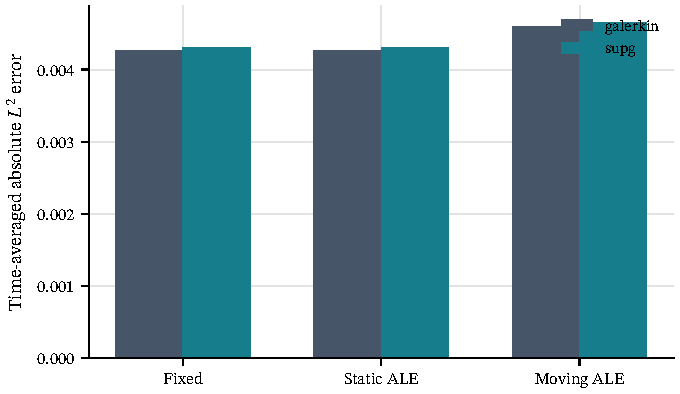
\includegraphics[width=0.95\columnwidth,height=0.29\textheight,keepaspectratio]{images/stage_e/supg_comparison.pdf}%
}{%
  \fbox{\begin{minipage}[c][0.105\textheight][c]{0.88\columnwidth}
  \centering\footnotesize\textbf{Figura non inclusa nel pacchetto sorgente}\par\vspace{0.35em}
  \scriptsize\nolinkurl{images/stage_e/supg_comparison.pdf}
  \end{minipage}}%
}
\caption{Confronto Galerkin/SUPG per mesh fissa, ALE statico e ALE mobile nella configurazione E1.}
\label{fig:e1_supg}
\end{figure}

\subsection{Verifica indipendente della D-GCL}

Per una traiettoria nodale affine in ogni passo, la mappa elementare è affine nel tempo e in due dimensioni $\det F(t)$ è un polinomio al più quadratico; la sua derivata è quindi lineare. Con elementi affini $P_1$, velocità nodale costante nel singolo intervallo, orientazione positiva per tutto il passo e quadratura esatta dei contributi geometrici (grado spaziale almeno due), la regola del punto medio integra esattamente la derivata temporale della matrice di massa. Il risultato è formulato come Lemma~\ref{lem:dgcl_midpoint} nell'Appendice~\ref{app:stageef}; si tratta di un'identità geometrica discreta sotto ipotesi precise, non di un teorema di stabilità o convergenza dello schema ALE. Nel test strutturato $16\times16$, il residuo element-wise nativo massimo è $8.69\times10^{-17}$ e il residuo algebrico in norma infinito è $4.63\times10^{-16}$. Il test free-stream ha errore $L^\infty$ pari a $4.10\times10^{-13}$. Il residuo lineare misurato è $1.13\times10^{-12}$, circa il 4.97\% della tolleranza GMRES effettiva riportata dal core. L'errore free-stream $4.10\times10^{-13}$ non coincide con il residuo geometrico (dell'ordine di $10^{-16}$): è misurato dopo l'assemblaggio e la soluzione del sistema discreto e include il contributo della soluzione lineare in precisione finita e dell'accumulo degli arrotondamenti. I valori riguardano la singola configurazione indipendente; non sostituiscono una verifica del bilancio integrale della PDE forzata.

\begin{table}[tbp]
\centering\small
\caption{Diagnostiche D-GCL della verifica indipendente Stage E1 su griglia strutturata $16\times16$.}
\label{tab:e1_dgcl}
\begin{tabular}{lr}
\toprule
Quantità & Valore\\
\midrule
Residuo element-wise nativo massimo & $8.69\times10^{-17}$\\
Residuo algebrico $L^\infty$ & $4.63\times10^{-16}$\\
Errore free-stream $L^\infty$ & $4.10\times10^{-13}$\\
Residuo lineare & $1.13\times10^{-12}$\\
Tolleranza GMRES effettiva & $2.27\times10^{-11}$\\
Rapporto residuo/tolleranza & 0.0497\\
\bottomrule
\end{tabular}
\end{table}

\subsection{Work--precision su mesh fisse}

La curva work--precision E1 usa $\Delta t=0.0025$ per tutte le griglie, un warm-up escluso e cinque ripetizioni temporali. Il tempo riportato è la mediana dei run di timing; l'errore è calcolato da una traiettoria di accuratezza dedicata, non dalle ripetizioni temporali. L'errore assoluto $L^2$ medio nel tempo passa da $1.074\times10^{-2}$ su $16^2$ a $3.048\times10^{-3}$ su $64^2$, mentre il tempo mediano cresce da 0.059 a 0.735 s. Poiché il passo temporale è mantenuto fisso e la contaminazione a $64^2$ supera il 10\%, questa curva è descritta come benchmark operativo a passo temporale fissato, non come curva di convergenza puramente spaziale.

\begin{table}[tbp]
\centering\small
\caption{Work--precision Galerkin a passo temporale fissato $\Delta t=0.0025$. Il tempo è la mediana di cinque misure, con un warm-up escluso.}
\label{tab:e1_wp}
\begin{tabular}{rrrr}
\toprule
Griglia & DOF & $\overline E_{L^2}^{\rm abs}$ & Tempo [s]\\
\midrule
$16^2$ & 289  & $1.074\times10^{-2}$ & 0.059\\
$32^2$ & 1089 & $4.262\times10^{-3}$ & 0.200\\
$64^2$ & 4225 & $3.048\times10^{-3}$ & 0.735\\
\bottomrule
\end{tabular}
\end{table}

\begin{figure*}[!t]
\centering
\IfFileExists{images/stage_e/fixed_grid_work_precision.pdf}{%
  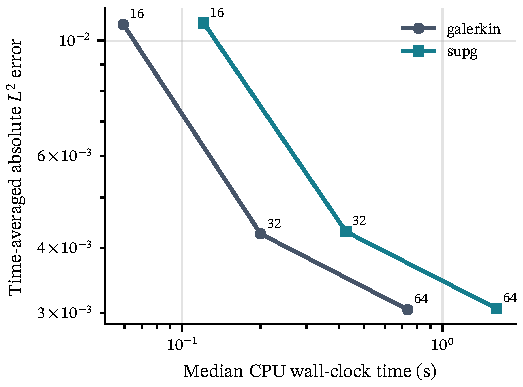
\includegraphics[width=0.95\textwidth,height=0.35\textheight,keepaspectratio]{images/stage_e/fixed_grid_work_precision.pdf}%
}{%
  \fbox{\begin{minipage}[c][0.105\textheight][c]{0.88\textwidth}
  \centering\footnotesize\textbf{Figura non inclusa nel pacchetto sorgente}\par\vspace{0.35em}
  \scriptsize\nolinkurl{images/stage_e/fixed_grid_work_precision.pdf}
  \end{minipage}}%
}
\caption{Work--precision Galerkin su mesh fisse a passo temporale costante. La curva è un benchmark operativo e non isola completamente l'errore spaziale al livello $64\times64$.}
\label{fig:e1_work_precision}
\end{figure*}

\subsection{Portata della verifica numerica e ALE}

E1 documenta un ordine temporale prossimo a uno su mesh fissa, ordini spaziali compatibili con $P_1$ sulla coppia $16^2$--$32^2$, equivalenza tra i percorsi fixed e ALE statico e consistenza D-GCL nel test indipendente specificato. Non documenta invece la convergenza del solutore su una famiglia di mesh mobili: la prova armonica ALE è una singola configurazione di deformazione e mostra un errore maggiore del caso fisso corrispondente. Inoltre, i risultati a $\Delta t=0.0025$ della prova SUPG e del work--precision non sono direttamente confrontabili con la campagna F1, che usa $\Delta t=0.005$. E1 non fornisce quindi una stima dell'errore temporale del benchmark F1 né dimostra che il suo guadagno sia puramente spaziale.
